% Options for packages loaded elsewhere
\PassOptionsToPackage{unicode}{hyperref}
\PassOptionsToPackage{hyphens}{url}
\PassOptionsToPackage{dvipsnames,svgnames,x11names}{xcolor}
%
\documentclass[
  letterpaper,
  10pt,
  openany]{report}

\usepackage{amsmath,amssymb}
\usepackage{iftex}
\ifPDFTeX
  \usepackage[T1]{fontenc}
  \usepackage[utf8]{inputenc}
  \usepackage{textcomp} % provide euro and other symbols
\else % if luatex or xetex
  \usepackage{unicode-math}
  \defaultfontfeatures{Scale=MatchLowercase}
  \defaultfontfeatures[\rmfamily]{Ligatures=TeX,Scale=1}
\fi
\usepackage{lmodern}
\ifPDFTeX\else  
    % xetex/luatex font selection
    \setmainfont[]{Georgia}
    \setsansfont[]{Calibri}
    \setmonofont[]{Consolas}
\fi
% Use upquote if available, for straight quotes in verbatim environments
\IfFileExists{upquote.sty}{\usepackage{upquote}}{}
\IfFileExists{microtype.sty}{% use microtype if available
  \usepackage[]{microtype}
  \UseMicrotypeSet[protrusion]{basicmath} % disable protrusion for tt fonts
}{}
\makeatletter
\@ifundefined{KOMAClassName}{% if non-KOMA class
  \IfFileExists{parskip.sty}{%
    \usepackage{parskip}
  }{% else
    \setlength{\parindent}{0pt}
    \setlength{\parskip}{6pt plus 2pt minus 1pt}}
}{% if KOMA class
  \KOMAoptions{parskip=half}}
\makeatother
\usepackage{xcolor}
\usepackage[top=25mm,left=18mm,right=18mm,bottom=20mm,heightrounded]{geometry}
\setlength{\emergencystretch}{3em} % prevent overfull lines
\setcounter{secnumdepth}{5}

\usepackage{color}
\usepackage{fancyvrb}
\newcommand{\VerbBar}{|}
\newcommand{\VERB}{\Verb[commandchars=\\\{\}]}
\DefineVerbatimEnvironment{Highlighting}{Verbatim}{commandchars=\\\{\}}
% Add ',fontsize=\small' for more characters per line
\usepackage{framed}
\definecolor{shadecolor}{RGB}{241,243,245}
\newenvironment{Shaded}{\begin{snugshade}}{\end{snugshade}}
\newcommand{\AlertTok}[1]{\textcolor[rgb]{0.68,0.00,0.00}{#1}}
\newcommand{\AnnotationTok}[1]{\textcolor[rgb]{0.37,0.37,0.37}{#1}}
\newcommand{\AttributeTok}[1]{\textcolor[rgb]{0.40,0.45,0.13}{#1}}
\newcommand{\BaseNTok}[1]{\textcolor[rgb]{0.68,0.00,0.00}{#1}}
\newcommand{\BuiltInTok}[1]{\textcolor[rgb]{0.00,0.23,0.31}{#1}}
\newcommand{\CharTok}[1]{\textcolor[rgb]{0.13,0.47,0.30}{#1}}
\newcommand{\CommentTok}[1]{\textcolor[rgb]{0.37,0.37,0.37}{#1}}
\newcommand{\CommentVarTok}[1]{\textcolor[rgb]{0.37,0.37,0.37}{\textit{#1}}}
\newcommand{\ConstantTok}[1]{\textcolor[rgb]{0.56,0.35,0.01}{#1}}
\newcommand{\ControlFlowTok}[1]{\textcolor[rgb]{0.00,0.23,0.31}{\textbf{#1}}}
\newcommand{\DataTypeTok}[1]{\textcolor[rgb]{0.68,0.00,0.00}{#1}}
\newcommand{\DecValTok}[1]{\textcolor[rgb]{0.68,0.00,0.00}{#1}}
\newcommand{\DocumentationTok}[1]{\textcolor[rgb]{0.37,0.37,0.37}{\textit{#1}}}
\newcommand{\ErrorTok}[1]{\textcolor[rgb]{0.68,0.00,0.00}{#1}}
\newcommand{\ExtensionTok}[1]{\textcolor[rgb]{0.00,0.23,0.31}{#1}}
\newcommand{\FloatTok}[1]{\textcolor[rgb]{0.68,0.00,0.00}{#1}}
\newcommand{\FunctionTok}[1]{\textcolor[rgb]{0.28,0.35,0.67}{#1}}
\newcommand{\ImportTok}[1]{\textcolor[rgb]{0.00,0.46,0.62}{#1}}
\newcommand{\InformationTok}[1]{\textcolor[rgb]{0.37,0.37,0.37}{#1}}
\newcommand{\KeywordTok}[1]{\textcolor[rgb]{0.00,0.23,0.31}{\textbf{#1}}}
\newcommand{\NormalTok}[1]{\textcolor[rgb]{0.00,0.23,0.31}{#1}}
\newcommand{\OperatorTok}[1]{\textcolor[rgb]{0.37,0.37,0.37}{#1}}
\newcommand{\OtherTok}[1]{\textcolor[rgb]{0.00,0.23,0.31}{#1}}
\newcommand{\PreprocessorTok}[1]{\textcolor[rgb]{0.68,0.00,0.00}{#1}}
\newcommand{\RegionMarkerTok}[1]{\textcolor[rgb]{0.00,0.23,0.31}{#1}}
\newcommand{\SpecialCharTok}[1]{\textcolor[rgb]{0.37,0.37,0.37}{#1}}
\newcommand{\SpecialStringTok}[1]{\textcolor[rgb]{0.13,0.47,0.30}{#1}}
\newcommand{\StringTok}[1]{\textcolor[rgb]{0.13,0.47,0.30}{#1}}
\newcommand{\VariableTok}[1]{\textcolor[rgb]{0.07,0.07,0.07}{#1}}
\newcommand{\VerbatimStringTok}[1]{\textcolor[rgb]{0.13,0.47,0.30}{#1}}
\newcommand{\WarningTok}[1]{\textcolor[rgb]{0.37,0.37,0.37}{\textit{#1}}}

\providecommand{\tightlist}{%
  \setlength{\itemsep}{0pt}\setlength{\parskip}{0pt}}\usepackage{longtable,booktabs,array}
\usepackage{calc} % for calculating minipage widths
% Correct order of tables after \paragraph or \subparagraph
\usepackage{etoolbox}
\makeatletter
\patchcmd\longtable{\par}{\if@noskipsec\mbox{}\fi\par}{}{}
\makeatother
% Allow footnotes in longtable head/foot
\IfFileExists{footnotehyper.sty}{\usepackage{footnotehyper}}{\usepackage{footnote}}
\makesavenoteenv{longtable}
\usepackage{graphicx}
\makeatletter
\def\maxwidth{\ifdim\Gin@nat@width>\linewidth\linewidth\else\Gin@nat@width\fi}
\def\maxheight{\ifdim\Gin@nat@height>\textheight\textheight\else\Gin@nat@height\fi}
\makeatother
% Scale images if necessary, so that they will not overflow the page
% margins by default, and it is still possible to overwrite the defaults
% using explicit options in \includegraphics[width, height, ...]{}
\setkeys{Gin}{width=\maxwidth,height=\maxheight,keepaspectratio}
% Set default figure placement to htbp
\makeatletter
\def\fps@figure{htbp}
\makeatother

\makeatletter
\@ifpackageloaded{tcolorbox}{}{\usepackage[skins,breakable]{tcolorbox}}
\@ifpackageloaded{fontawesome5}{}{\usepackage{fontawesome5}}
\definecolor{quarto-callout-color}{HTML}{909090}
\definecolor{quarto-callout-note-color}{HTML}{0758E5}
\definecolor{quarto-callout-important-color}{HTML}{CC1914}
\definecolor{quarto-callout-warning-color}{HTML}{EB9113}
\definecolor{quarto-callout-tip-color}{HTML}{00A047}
\definecolor{quarto-callout-caution-color}{HTML}{FC5300}
\definecolor{quarto-callout-color-frame}{HTML}{acacac}
\definecolor{quarto-callout-note-color-frame}{HTML}{4582ec}
\definecolor{quarto-callout-important-color-frame}{HTML}{d9534f}
\definecolor{quarto-callout-warning-color-frame}{HTML}{f0ad4e}
\definecolor{quarto-callout-tip-color-frame}{HTML}{02b875}
\definecolor{quarto-callout-caution-color-frame}{HTML}{fd7e14}
\makeatother
\makeatletter
\@ifpackageloaded{bookmark}{}{\usepackage{bookmark}}
\makeatother
\makeatletter
\@ifpackageloaded{caption}{}{\usepackage{caption}}
\AtBeginDocument{%
\ifdefined\contentsname
  \renewcommand*\contentsname{Зміст}
\else
  \newcommand\contentsname{Зміст}
\fi
\ifdefined\listfigurename
  \renewcommand*\listfigurename{Список рисунків}
\else
  \newcommand\listfigurename{Список рисунків}
\fi
\ifdefined\listtablename
  \renewcommand*\listtablename{Список таблиць}
\else
  \newcommand\listtablename{Список таблиць}
\fi
\ifdefined\figurename
  \renewcommand*\figurename{Рисунок}
\else
  \newcommand\figurename{Рисунок}
\fi
\ifdefined\tablename
  \renewcommand*\tablename{Таблиця}
\else
  \newcommand\tablename{Таблиця}
\fi
}
\@ifpackageloaded{float}{}{\usepackage{float}}
\floatstyle{ruled}
\@ifundefined{c@chapter}{\newfloat{codelisting}{h}{lop}}{\newfloat{codelisting}{h}{lop}[chapter]}
\floatname{codelisting}{Лістинг}
\newcommand*\listoflistings{\listof{codelisting}{Список каталогів}}
\usepackage{amsthm}
\theoremstyle{definition}
\newtheorem{example}{Приклад}[chapter]
\theoremstyle{remark}
\AtBeginDocument{\renewcommand*{\proofname}{Доведення}}
\newtheorem*{remark}{Примітка}
\newtheorem*{solution}{Рішення}
\newtheorem{refremark}{Примітка}[chapter]
\newtheorem{refsolution}{Рішення}[chapter]
\makeatother
\makeatletter
\makeatother
\makeatletter
\@ifpackageloaded{caption}{}{\usepackage{caption}}
\@ifpackageloaded{subcaption}{}{\usepackage{subcaption}}
\makeatother
\makeatletter
\@ifpackageloaded{tikz}{}{\usepackage{tikz}}
\makeatother
        \newcommand*\circled[1]{\tikz[baseline=(char.base)]{
          \node[shape=circle,draw,inner sep=1pt] (char) {{\scriptsize#1}};}}  
                  

\ifLuaTeX
  \usepackage{selnolig}  % disable illegal ligatures
\fi
\usepackage{bookmark}

\IfFileExists{xurl.sty}{\usepackage{xurl}}{} % add URL line breaks if available
\urlstyle{same} % disable monospaced font for URLs
\hypersetup{
  pdftitle={Прикладний статистичний аналіз},
  pdfauthor={Ігор Мірошниченко; Юлія Хлевна},
  colorlinks=true,
  linkcolor={blue},
  filecolor={Maroon},
  citecolor={Blue},
  urlcolor={Blue},
  pdfcreator={LaTeX via pandoc}}


\title{Прикладний статистичний аналіз}
\author{Ігор Мірошниченко \and Юлія Хлевна}
\date{2025-03-26}

\begin{document}
\maketitle

\renewcommand*\contentsname{Зміст}
{
\hypersetup{linkcolor=}
\setcounter{tocdepth}{1}
\tableofcontents
}

\bookmarksetup{startatroot}

\chapter*{Передмова}\label{ux43fux435ux440ux435ux434ux43cux43eux432ux430}
\addcontentsline{toc}{chapter}{Передмова}

\markboth{Передмова}{Передмова}

\bookmarksetup{startatroot}

\chapter*{Вступ}\label{sec-intro}
\addcontentsline{toc}{chapter}{Вступ}

\markboth{Вступ}{Вступ}

\bookmarksetup{startatroot}

\chapter{Біноміальний критерій}\label{sec-binom}

\section{Генеральна сукупність та
вибірка}\label{ux433ux435ux43dux435ux440ux430ux43bux44cux43dux430-ux441ux443ux43aux443ux43fux43dux456ux441ux442ux44c-ux442ux430-ux432ux438ux431ux456ux440ux43aux430}

Ви вирішили створити платформу онлайн-курсів з програмування. Ви
записали навчальні відео та запропонували користувачам доступ за
передплатою. Вартість курсу для студента становить 1000 гривень, а
витрати на підтримку платформи та індивідуальні консультації коштують
вам 500 гривень з кожного студента.

Проте ви помічаєте, що деякі люди відмовляються від курсу після першого
заняття, якщо матеріал їм здається складним або нецікавим. Інвестори
готові підтримати ваш проєкт, якщо рівень відмов буде нижче 50\%.

Щоб це перевірити, ви проводите експеримент: залучаєте 30 нових
студентів. 20 із них проходять курс й оплачують доступ, а 11
відмовляються. 20 --- це більше половини, але чи достатньо цього, щоб
довести перспективність проєкту?

Розв'язуючи таку задачу, ми припускаємо, що існує певна аудиторія, яка
користуватиметься нашим сервісом. Цю групу називають \textbf{генеральною
сукупністю}. Якщо запустити сервіс для всіх потенційних користувачів, у
ньому буде певна частка успішних випадків, позначимо її як \(\mu\). Це
невідомий параметр, який ми не можемо визначити безпосередньо. Натомість
ми можемо проводити експерименти та \textbf{досліджувати} результати.
Оскільки протестувати продукт на всій аудиторії неможливо, ми беремо
\textbf{вибірку} з генеральної сукупності та аналізуємо частку успішних
випадків.

Згідно з результатами нашого експерименту, спостережувана ймовірність
оплати становить \(\hat{\mu} = 20/30 = 0.67\)\footnote{У статистиці
  \(\hat{\mu}\) позначається як оцінка параметра \(\mu\).}. Це означає,
що 67\% студентів оплатили доступ. Чи можемо ми зробити висновок, що
справжня частка успішних випадків перевищує 50\%?

Розгляньмо, чому отримане значення \emph{може не бути} переконливим
доказом. Припустимо, що ймовірність успішної оплати дорівнює
\(\mu = 0.5\), і змоделюємо можливі результати для 30 студентів.

Давайте спростимо цю задачу до прикладу з підкиданням монетки та
змоделюємо результати для 30 спроб:

\begin{itemize}
\tightlist
\item
  Якщо монетка випаде орлом, студент оплачує доступ.
\item
  Якщо монетка випаде решкою, студент відмовляється від курсу.
\item
  Використаємо метод \texttt{integers()} до класу \texttt{Generator},
  яка генерує випадкові цілі числа в заданому діапазоні.
\item
  Підкинемо монетку 30 разів та порахуємо кількість успішних випадків.
\end{itemize}

\phantomsection\label{annotated-cell-1}%
\begin{Shaded}
\begin{Highlighting}[]
\NormalTok{rng }\OperatorTok{=}\NormalTok{ np.random.default\_rng(}\DecValTok{18}\NormalTok{) }\hspace*{\fill}\NormalTok{\circled{1}}

\NormalTok{n }\OperatorTok{=} \DecValTok{30} \hspace*{\fill}\NormalTok{\circled{2}}
\NormalTok{results }\OperatorTok{=}\NormalTok{ rng.integers(}\DecValTok{0}\NormalTok{, }\DecValTok{1}\NormalTok{, size }\OperatorTok{=} \DecValTok{30}\NormalTok{, endpoint }\OperatorTok{=} \VariableTok{True}\NormalTok{) }\hspace*{\fill}\NormalTok{\circled{3}}
\NormalTok{success }\OperatorTok{=}\NormalTok{ np.}\BuiltInTok{sum}\NormalTok{(results) }\OperatorTok{/}\NormalTok{ n }\hspace*{\fill}\NormalTok{\circled{4}}

\BuiltInTok{print}\NormalTok{(}\SpecialStringTok{f"Кількість успішних випадків: }\SpecialCharTok{\{}\BuiltInTok{round}\NormalTok{(success, }\DecValTok{3}\NormalTok{) }\OperatorTok{*} \DecValTok{100}\SpecialCharTok{\}}\SpecialStringTok{\%"}\NormalTok{) }\hspace*{\fill}\NormalTok{\circled{5}}
\end{Highlighting}
\end{Shaded}

\begin{description}
\tightlist
\item[\circled{1}]
Ініціалізуємо генератор випадкових чисел з фіксованим \texttt{seed}.
\item[\circled{2}]
Кількість студентів.
\item[\circled{3}]
Генеруємо випадкові числа\footnote{Метод \texttt{integers()} генерує
  випадкові цілі числа в заданому діапазоні. Аргумент \texttt{endpoint}
  вказує, що верхня межа включається у діапазон.} для кожного студента.
\item[\circled{4}]
Обчислюємо частку успішних випадків.
\item[\circled{5}]
Виводимо результат.
\end{description}

\begin{verbatim}
Кількість успішних випадків: 70.0%
\end{verbatim}

Ми бачимо, що в експерименті частка успішних випадків навіть перевищила
63\%, тоді як у симуляції була закладена ймовірність 50\%.

Тому, на жаль, ми не можемо з абсолютною точністю визначити, яким є
справжнє значення \(\mu\) у генеральній сукупності та чи перевищує воно
50\%, незалежно від того, скільки спостережень ми проводимо. Однак,
застосовуючи методи прикладної статистики, ми зможемо використати
інструменти, які допоможуть ухвалити правильне рішення, зокрема й у
цьому випадку.

\section{Статистичні
гіпотези}\label{ux441ux442ux430ux442ux438ux441ux442ux438ux447ux43dux456-ux433ux456ux43fux43eux442ux435ux437ux438}

\subsection{Постановка
задачі}\label{ux43fux43eux441ux442ux430ux43dux43eux432ux43aux430-ux437ux430ux434ux430ux447ux456}

Ми з'ясували, що навіть за ймовірності \(\mu = 0.5\) можна отримати
значну кількість успішних випадків. Насправді ми спеціально підбирали
\texttt{seed} для отримання такого результату. Якщо повторити цей
експеримент з іншим значенням \texttt{seed} або збільшити кількість
спостережень, результат може виявитися іншим.

\begin{tcolorbox}[enhanced jigsaw, colframe=quarto-callout-tip-color-frame, colback=white, colbacktitle=quarto-callout-tip-color!10!white, opacityback=0, toprule=.15mm, bottomtitle=1mm, toptitle=1mm, leftrule=.75mm, rightrule=.15mm, breakable, opacitybacktitle=0.6, arc=.35mm, titlerule=0mm, coltitle=black, bottomrule=.15mm, left=2mm, title=\textcolor{quarto-callout-tip-color}{\faLightbulb}\hspace{0.5em}{Порада}]

Спробуйте змінити \texttt{seed} (наприклад 22) або кількість
спостережень та перевірте, як змінюється результат.

\end{tcolorbox}

Тож велика кількість успішних випадків може бути результатом
випадковості. Щоб вирішити, чи можна вважати результати експерименту
\textbf{статистично значущими} необхідно отримати відповідь на питання:

\begin{quote}
Чи можна вважати, що спостережуване значення \(\hat{\mu}\) є більшим від
\(\mu = 0.5\)?
\end{quote}

Звернімося до теорії ймовірностей. Факт підписки на наш сервіс для
кожного окремого студента можна розглядати як випадкову величину
\(\xi\), яка підпорядковується розподілу Бернуллі\footnote{Розподіл
  Бернуллі --- це дискретний розподіл ймовірностей, який моделює
  випадковий експеримент з двома можливими результатами: успіхом або
  невдачею.}. Параметр цього розподілу, а саме ймовірність успіху, нам
невідомий.

\[
\xi \sim \text{Bernoulli}(\mu)
\]

де \(\mu\) --- ймовірність успіху.

Нас цікавить підтвердження того, що \(\mu > 0.5\). У статистиці для
перевірки гіпотез розглядають дві можливості:

\begin{itemize}
\tightlist
\item
  \textbf{Нульова гіпотеза} (\(H_0\)) формулюється як твердження, яке ми
  прагнемо спростувати.
\item
  \textbf{Альтернативна гіпотеза} (\(H_1\)) висловлює припущення, яке ми
  хочемо довести.
\end{itemize}

Скорочено це записують як:

\[
\begin{aligned}
H_0 &: \mu \leq 0.5 \\
H_1 &: \mu > 0.5
\end{aligned}
\]

Зауважимо, що якщо в нашому експерименті з 30 студентами можна дивитися
не на частку успіхів, а на їх \textbf{кількість}.

Тоді питання можна переформулювати так:

\begin{quote}
За умови вірності \(H_0\) наскільки ймовірно отримати 20 або більше
успішних випадків з 30?
\end{quote}

Якщо ми проводимо \(n\) незалежних спостережень, то сума цих випадкових
величин також підпорядковується біноміальному розподілу\footnote{Біноміальний
  розподіл моделює кількість успішних випадків у послідовності
  незалежних випробувань. Сума \(n\) незалежних випадкових величин з
  розподілу Бернуллі підпорядковується біноміальному розподілу.}.

\[
S_n = \sum_{i=1}^{n} \xi_i \sim \text{Binomial}(n, \mu)
\]

де \(\xi_i\) --- випадкова величина, яка показує успіх у \(i\)-му
спостереженні, \(S_n\) --- кількість успішних випадків у \(n\)
спостереженнях, \(n\) --- кількість спостережень, \(\mu\) ---
ймовірність успіху.

Давайте подивимось, як це виглядає графічно. Для цього побудуємо графік
функції щільності ймовірностей для біноміального розподілу з параметрами
\(n = 30\) та \(\mu = 0.5\).

\begin{Shaded}
\begin{Highlighting}[]
\NormalTok{n }\OperatorTok{=} \DecValTok{30}
\NormalTok{mu }\OperatorTok{=} \FloatTok{0.5}

\NormalTok{x }\OperatorTok{=}\NormalTok{ np.arange(}\DecValTok{0}\NormalTok{, n }\OperatorTok{+} \DecValTok{1}\NormalTok{)}
\NormalTok{y }\OperatorTok{=}\NormalTok{ binom.pmf(x, n, mu)}

\NormalTok{plt.bar(x, y, color}\OperatorTok{=}\NormalTok{turquoise)}
\NormalTok{plt.bar(x[x }\OperatorTok{\textgreater{}=} \DecValTok{20}\NormalTok{], y[x }\OperatorTok{\textgreater{}=} \DecValTok{20}\NormalTok{], color}\OperatorTok{=}\NormalTok{red\_pink)}
\NormalTok{plt.xlabel(}\StringTok{"Кількість успішних випадків"}\NormalTok{)}
\NormalTok{plt.ylabel(}\StringTok{"Ймовірність"}\NormalTok{)}
\NormalTok{plt.show()}
\end{Highlighting}
\end{Shaded}

\begin{figure}[H]

\centering{

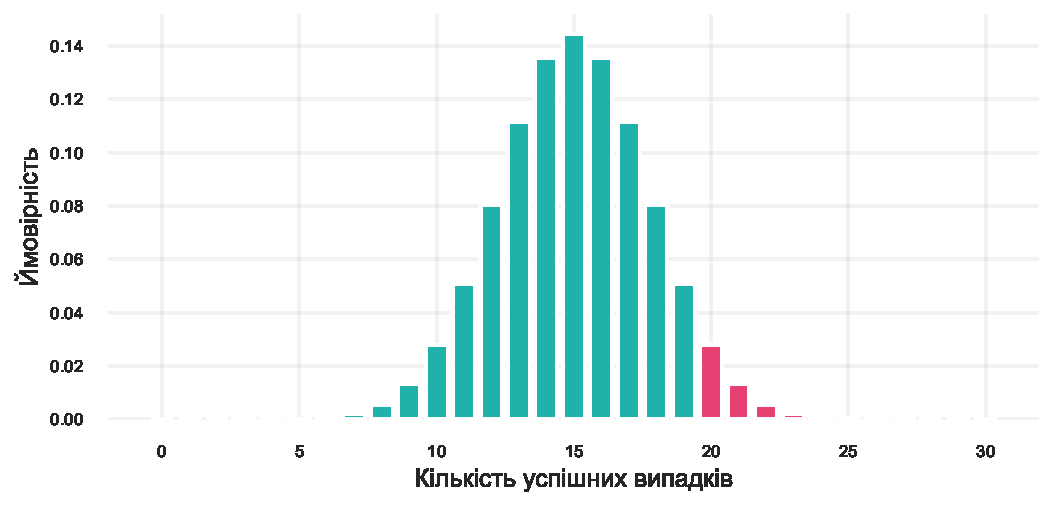
\includegraphics{binom_files/figure-pdf/fig-binom-pmf-output-1.pdf}

}

\caption{\label{fig-binom-pmf}Функція щільності ймовірностей при
\(H_0\)}

\end{figure}%

Рисунок~\ref{fig-binom-pmf} демонструє функцію щільності ймовірностей
для біноміального розподілу з параметрами \(n = 30\) та \(\mu = 0.5\).
Ціановим\footnote{Англ. \emph{cyan}, від грец. κυανoῦς ---
  ``блакитний'', ``лазуровий''.} кольором позначено ймовірності для
кожної кількості успішних випадків. Рожевими виділено ймовірності для
кількості успішних випадків, яка перевищує або дорівнює 20.

\subsection{Критерій}\label{ux43aux440ux438ux442ux435ux440ux456ux439}

Щойно ми розробили алгоритм, який на основі вибірки \(\xi\) або визнає
наявність доказів на користь \(H_1\), або повідомляє, що таких доказів
немає. Відповідно, він або відхиляє \(H_0\), або не відхиляє її.

Такий алгоритм називається \textbf{критерієм}. Його можна подати у
вигляді функції \(S\), яка приймає реалізацію вибірки та повертає \(1\),
якщо слід відхилити \(H_0\), та \(0\) в іншому випадку.

\[
S(\xi) = \begin{cases}
    1, \text{ якщо відхиляємо } H_0 \\
    0, \text{ в іншому випадку}
\end{cases}
\]

Давайте припустимо, що ми вирішили відхилити \(H_0\), якщо кількість
успішних випадків перевищує або дорівнює 21. Тоді критерій набуде
вигляду:

\[
S(\xi) = \begin{cases}
    1, \text{ якщо } \sum \xi_i \geqslant 21 \\
    0, \text{ в іншому випадку}
\end{cases}
\]

Зазвичай скорочують запис і пишуть просто правило, за яким відхиляємо
\(H_0\)

\[
S = \{\sum \xi_i \geqslant 21\} 
\]

Позначимо \(Q = \sum \xi_i\), \(C = 21\), тоді критерій набуває вигляду:

\[
S = \{Q(\xi) \geqslant C\} 
\]

Так влаштована більшість класичних критеріїв у прикладній статистиці,
тому величинам у ньому дано спеціальні назви. \(Q\) називається
\textbf{статистикою критерію}, \(C\) --- \textbf{критичним значенням}.

\(Q\) може бути будь-якою функцією від вибірки, яку ви вважаєте логічною
для перевірки гіпотези. У нашому випадку це кількість успіхів, або сума
всіх \(\xi_i\). Але ви можете вибрати й інші: максимальне значення, суму
перших 5 значень або навіть просто перший елемент.

\subsection{Критична
область}\label{ux43aux440ux438ux442ux438ux447ux43dux430-ux43eux431ux43bux430ux441ux442ux44c}

Знову перепишемо наше основне запитання, тільки тепер з використанням
нашого критерію \(S\):

\begin{quote}
Наскільки часто може бути таке, що за справедливості \(H_0\) критерій
\(S\) відхиляє гіпотезу?
\end{quote}

Відповідь на це запитання залежить від критичного значення. Зараз ми
взяли його рівним 21, побачивши на картинці, що великі відхилення
відбуваються при \(H_0\) рідко. Але що означає рідко й наскільки рідко,
не сказали. Тепер наша мета зрозуміти, як вибрати критичне значення
\(C\), виходячи з \textbf{частоти помилок} нашого критерію.

Вибираючи \(C\), ми можемо або часто відхиляти нульову гіпотезу, коли
\(C\) мале, або можемо робити це рідше, коли \(C\) велике. Щоб вибрати
правильне значення, потрібно визначитися, коли наш критерій помиляється.

\begin{itemize}
\item
  \(C = 16\). Якщо відхиляти гіпотезу при отриманні хоча б 16 успішних
  підписок із 30, то це навряд чи влаштує інвесторів. Так, успіхів
  більше половини. Але якщо в генеральній сукупності ймовірність 0.5, то
  майже в половині випадків ми будемо відхиляти гіпотезу. Критерій
  помилково повертає \(1\), тобто це помилка \textbf{хибно позитивна}
  (false positive, \textbf{FP}).
\item
  \(C = 29\). У такому разі будемо відхиляти гіпотезу тільки за 29 або
  30 успіхів. Ці значення, звісно, говорять про те, що відхилення від
  50\% успіхів сильне. Але якщо в генеральній сукупності ймовірність,
  наприклад, 60\%, то такі значення будуть виходити рідко. Але ж такі
  ймовірності теж влаштували б інвесторів, й ми б змогли відкрити
  стартап! А з таким критерієм ми навряд чи доб'ємося цього. Не
  відхилити гіпотезу \(H_0\), коли вона неправильна --- це теж помилка.
  Вона називається \textbf{хибно негативна} (false negative,
  \textbf{FN}), оскільки критерій повернув 0 помилково.
\end{itemize}

\[ \text{FP} - H_0\ відхиляється,\ коли\ вона\ вірна \]
\[ \text{FN} - H_0\ не\ відхиляється,\ коли\ вона\ не вірна \]

У нашому завданні інвесторам важливіше хибно позитивна помилка. Їм дуже
не хочеться потрапити в ситуацію, коли їм показали доказ успішності
бізнесу, а виявилося, більшість користувачів відмовляється оформлювати
підписку й компанія не отримує прибуток. Це призведе до збитків. Хибно
негативна помилка призведе до того, що ви втратите успішний бізнес, але
інвестори грошей не втратять.

Тому виберемо поріг, щоб ймовірність хибно позитивної помилки була
задовільною, або ж \textbf{частота хибнопозитивних спрацьовувань} (False
Positive Rate, FPR). Для цього треба зрозуміти, як часто ми будемо
відхиляти гіпотезу, за умови вірності \(H_0\).

Тепер знову переформулюємо основне питання, повністю з використанням
нових термінів, й врешті-решт відповімо на нього.

\begin{quote}
Який FPR у критерію \(S\) для перевірки гіпотези \(H_0\) проти \(H_1\)?
\end{quote}

Коли \(H_0\) є вірною, щоб порахувати кількість успіхів ми проводили 30
разів підкидання монетки з ймовірністю орла \(0.5\). Кількість орлів
(тобто успіхів) у такому експерименті має розподіл, який називається
біноміальним, тобто при \(\mu = 0.5\) наша статистика має біноміальний
розподіл \(Q \sim Binom(0.5, 30)\).

Обчислимо FPR для \(C = 21\)

\[
\begin{aligned}
FPR &= P(S(\xi) = 1\ |\ H_0) \\
&= P(Q \geqslant 21\ |\ H_0) \\
&= P(Q \geqslant 21\ |\ \mu = 0.5) = \\
&= P(Q \geqslant 21\ |\ Q \sim Binom(0.5, 30))
\end{aligned}
\]

Це вже ймовірність події за конкретного розподілу випадкової величини.
Його можна подивитися за таблицею або, що зручніше, обчислити з
використанням мов програмування.

\subsection{Обчислення
FPR}\label{ux43eux431ux447ux438ux441ux43bux435ux43dux43dux44f-fpr}

Давайте порахуємо суму ймовірностей для кількостей успіхів від 21 до 30
включно. Покажемо графічно, як це виглядає на
Рисунку~\ref{fig-binom-pmf-fpr}.

\begin{Shaded}
\begin{Highlighting}[]
\NormalTok{x }\OperatorTok{=}\NormalTok{ np.arange(}\DecValTok{0}\NormalTok{, n }\OperatorTok{+} \DecValTok{1}\NormalTok{)}
\NormalTok{y }\OperatorTok{=}\NormalTok{ binom.pmf(x, n, }\FloatTok{0.5}\NormalTok{)}

\NormalTok{plt.bar(x, y, color}\OperatorTok{=}\NormalTok{turquoise)}
\NormalTok{plt.bar(x[x }\OperatorTok{\textgreater{}=}\NormalTok{ crit\_subs], y[x }\OperatorTok{\textgreater{}=}\NormalTok{ crit\_subs], color}\OperatorTok{=}\NormalTok{red\_pink)}
\ControlFlowTok{for}\NormalTok{ i }\KeywordTok{in} \BuiltInTok{range}\NormalTok{(crit\_subs }\OperatorTok{{-}} \DecValTok{2}\NormalTok{, crit\_subs }\OperatorTok{+} \DecValTok{4}\NormalTok{):}
\NormalTok{    plt.text(i }\OperatorTok{+} \FloatTok{0.5}\NormalTok{, y[i] }\OperatorTok{+} \FloatTok{0.001}\NormalTok{, }\SpecialStringTok{f"}\SpecialCharTok{\{}\BuiltInTok{round}\NormalTok{(y[i] }\OperatorTok{*} \DecValTok{100}\NormalTok{, }\DecValTok{1}\NormalTok{)}\SpecialCharTok{\}}\SpecialStringTok{\%"}\NormalTok{,}
\NormalTok{    ha}\OperatorTok{=}\StringTok{\textquotesingle{}center\textquotesingle{}}\NormalTok{, va}\OperatorTok{=}\StringTok{\textquotesingle{}bottom\textquotesingle{}}\NormalTok{, size}\OperatorTok{=}\DecValTok{8}\NormalTok{, rotation }\OperatorTok{=} \DecValTok{30}\NormalTok{)}
\NormalTok{plt.xlabel(}\StringTok{"Кількість успішних випадків"}\NormalTok{)}
\NormalTok{plt.ylabel(}\StringTok{"Ймовірність"}\NormalTok{)}
\NormalTok{plt.show()}
\end{Highlighting}
\end{Shaded}

\begin{figure}[H]

\centering{

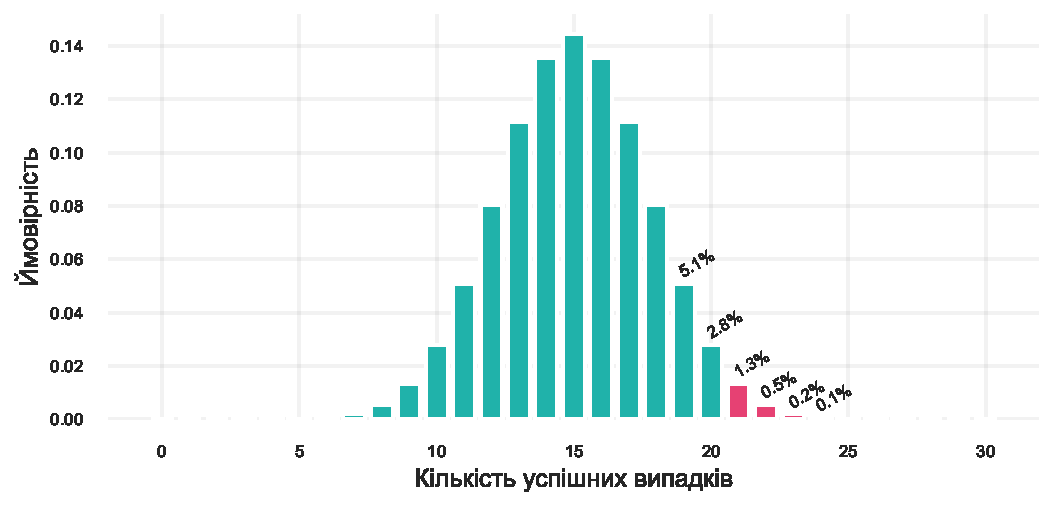
\includegraphics{binom_files/figure-pdf/fig-binom-pmf-fpr-output-1.pdf}

}

\caption{\label{fig-binom-pmf-fpr}Ймовірність хибно відхилити \(H_0\) за
умови її вірності}

\end{figure}%

Залишається лише обчислити суму ймовірностей для кількостей успіхів від
21 до 30 включно. Це і буде нашим FPR.

\[
FPR_{21} = \sum_{i = 21}^{30} P(Q = i) \approx 0.021
\]

У нашому випадку це буде 2.1\%. Якщо FPR не перевищує деякої константи
\(\alpha\), то критерій називається критерієм \textbf{рівня значущості}
\(\alpha\). Статистичний критерій з \(\alpha\) = 100\% створити
тривіально --- достатньо завжди відхиляти \(H_0\) --- тому така
постановка не має сенсу.

Рівень значущості зазвичай обирають на основі бізнес-міркувань. Він
позначає те, який ризик неправильного прийняття позитивного рішення ми
вважаємо прийнятним. Зазвичай беруть \(\alpha = 0.05\), але якщо
потрібне більш точне ухвалення рішення, можуть вибрати \(0.01\),
\(0.005\), \(0.001\). Якщо ж рішення не таке критичне, можуть вибрати
\(0.1\).

Припустимо, вибрали значення \(\alpha = 0.05\), скористаємося критерієм
\(S\): тобто якщо кількість успішних випадків перевищує або дорівнює 21,
то відхиляємо \(H_0\).

Якщо уважно подивитись на Рисунок~\ref{fig-binom-pmf-fpr}, то можна
помітити, що ми можемо відхиляти \(H_0\) при кількості успіхів від 20, а
не 21, оскільки такий все ще буде відповідати \(\alpha = 0.05\):

\[
FPR_{20} = \sum_{i = 20}^{30} P(Q = i) \approx 0.049
\]

Якщо ж обрати 19, то FPR буде більше \(\alpha\): \[
FPR_{19} = \sum_{i = 20}^{30} P(Q = i) \approx 0.1002
\]

\section{Статистичні функції в
Python}\label{ux441ux442ux430ux442ux438ux441ux442ux438ux447ux43dux456-ux444ux443ux43dux43aux446ux456ux457-ux432-python}

У цій частині подивимося, як вивести те, що ми отримали в частині 2, за
допомогою Python. А також зрозуміємо, як знайти відповідне \(C\) за
допомогою Python.

\subsection{Біноміальний
розподіл}\label{ux431ux456ux43dux43eux43cux456ux430ux43bux44cux43dux438ux439-ux440ux43eux437ux43fux43eux434ux456ux43b}

Ми з'ясували, що статистика \(Q\) має біноміальний розподіл.

Біноміальний розподіл \(Binom(n, \mu)\) --- розподіл кількості успіхів у
послідовності з \(n\) незалежних випадкових експериментів, ймовірність
успіху в кожному з яких дорівнює \(\mu\).

Щоб працювати з розподілом, можна створити об'єкт-розподіл за допомогою
бібліотеки \texttt{scipy.stats}.

\phantomsection\label{annotated-cell-4}%
\begin{Shaded}
\begin{Highlighting}[]
\ImportTok{from}\NormalTok{ scipy.stats }\ImportTok{import}\NormalTok{ binom}

\NormalTok{n }\OperatorTok{=} \DecValTok{30} \hspace*{\fill}\NormalTok{\circled{1}}
\NormalTok{mu }\OperatorTok{=} \FloatTok{0.5} \hspace*{\fill}\NormalTok{\circled{2}}

\NormalTok{binom\_dist }\OperatorTok{=}\NormalTok{ binom(n, mu)}
\end{Highlighting}
\end{Shaded}

\begin{description}
\tightlist
\item[\circled{1}]
Кількість спостережень.
\item[\circled{2}]
Ймовірність успіху.
\end{description}

\subsection{Функція
ймовірностей}\label{ux444ux443ux43dux43aux446ux456ux44f-ux439ux43cux43eux432ux456ux440ux43dux43eux441ux442ux435ux439}

Функція ймовірності дискретного розподілу \(p_\xi(x)\) --- ймовірність,
з якою \(\xi\) приймає значення \(x\).

У Python це функція \texttt{pmf} (probability mass function).

\phantomsection\label{annotated-cell-5}%
\begin{Shaded}
\begin{Highlighting}[]
\NormalTok{binom\_dist.pmf(}\DecValTok{20}\NormalTok{) }\hspace*{\fill}\NormalTok{\circled{1}}
\end{Highlighting}
\end{Shaded}

\begin{description}
\tightlist
\item[\circled{1}]
Ймовірність отримати 20 успішних випадків.
\end{description}

\begin{verbatim}
0.027981600724160654
\end{verbatim}

Зобразимо розподіл статистики \(Q\) за справедливості \(H_0\) на
графіку. Для цього можна передати відразу масив точок, для яких треба
розрахувати ймовірність.

\phantomsection\label{annotated-cell-6}%
\begin{Shaded}
\begin{Highlighting}[]
\NormalTok{x }\OperatorTok{=}\NormalTok{ np.arange(}\DecValTok{0}\NormalTok{, n }\OperatorTok{+} \DecValTok{1}\NormalTok{) }\hspace*{\fill}\NormalTok{\circled{1}}
\NormalTok{y }\OperatorTok{=}\NormalTok{ binom\_dist.pmf(x) }\hspace*{\fill}\NormalTok{\circled{2}}

\NormalTok{crit\_subs }\OperatorTok{=} \DecValTok{21} \hspace*{\fill}\NormalTok{\circled{3}}

\NormalTok{plt.bar(x, y, color}\OperatorTok{=}\NormalTok{turquoise, label}\OperatorTok{=}\StringTok{"Ймовірність успіхів"}\NormalTok{) }\hspace*{\fill}\NormalTok{\circled{4}}
\NormalTok{plt.bar(x[x }\OperatorTok{\textgreater{}=}\NormalTok{ crit\_subs], y[x }\OperatorTok{\textgreater{}=}\NormalTok{ crit\_subs], color}\OperatorTok{=}\NormalTok{red\_pink, label}\OperatorTok{=}\StringTok{"Критичне значення"}\NormalTok{) }\hspace*{\fill}\NormalTok{\circled{5}}
\NormalTok{plt.xlabel(}\StringTok{"Кількість успішних випадків"}\NormalTok{)}
\NormalTok{plt.ylabel(}\StringTok{"Ймовірність"}\NormalTok{)}
\NormalTok{plt.show()}
\end{Highlighting}
\end{Shaded}

\begin{description}
\tightlist
\item[\circled{1}]
Масив точок.
\item[\circled{2}]
Розрахунок ймовірностей.
\item[\circled{3}]
Критичне значення.
\item[\circled{4}]
Ймовірність успіхів.
\item[\circled{5}]
Критичне значення.
\end{description}

\begin{figure}[H]

\centering{

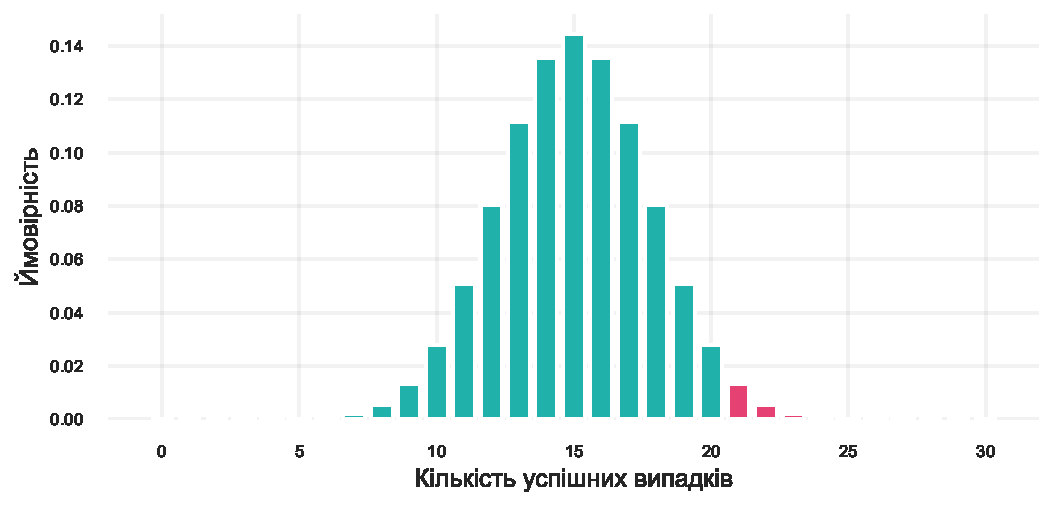
\includegraphics{binom_files/figure-pdf/fig-binom-pmf-python-output-1.pdf}

}

\caption{\label{fig-binom-pmf-python}Функція щільності ймовірностей
біноміального розподілу}

\end{figure}%

Насправді вже зараз ми можемо порахувати ймовірність потрапляння в
критичну область. Потрібно просто підсумувати ймовірності для кількостей
успіхів від 21 до 30.

\begin{Shaded}
\begin{Highlighting}[]
\NormalTok{np.}\BuiltInTok{round}\NormalTok{(np.}\BuiltInTok{sum}\NormalTok{(y[crit\_subs:]), }\DecValTok{4}\NormalTok{)}
\end{Highlighting}
\end{Shaded}

\begin{verbatim}
0.0214
\end{verbatim}

Отже, ми дійсно побудували критерій рівня значущості \(\alpha = 0.05\).
Ба більше, це критерій рівня значущості 0.021.

А що якби ми взяли \(C = 19\)?

\begin{Shaded}
\begin{Highlighting}[]
\NormalTok{crit\_subs }\OperatorTok{=} \DecValTok{19}
\NormalTok{np.}\BuiltInTok{round}\NormalTok{(np.}\BuiltInTok{sum}\NormalTok{(y[crit\_subs:]), }\DecValTok{4}\NormalTok{)}
\end{Highlighting}
\end{Shaded}

\begin{verbatim}
0.1002
\end{verbatim}

Тоді ймовірність помилки вже навіть більше \(10\%\), що зовсім нам не
підходить.

А якщо \(C = 20\)?

\begin{Shaded}
\begin{Highlighting}[]
\NormalTok{crit\_subs }\OperatorTok{=} \DecValTok{20}
\NormalTok{np.}\BuiltInTok{round}\NormalTok{(np.}\BuiltInTok{sum}\NormalTok{(y[crit\_subs:]), }\DecValTok{4}\NormalTok{)}
\end{Highlighting}
\end{Shaded}

\begin{verbatim}
0.0494
\end{verbatim}

Видно, що немає такого \(C\), щоб FPR був рівно \(5\%\).

\subsection{Кумулятивна функція
розподілу}\label{ux43aux443ux43cux443ux43bux44fux442ux438ux432ux43dux430-ux444ux443ux43dux43aux446ux456ux44f-ux440ux43eux437ux43fux43eux434ux456ux43bux443}

Кумулятивна функція розподілу \(F_\xi(x) = P(\xi \leqslant x)\)

У Python це функція \texttt{cdf} (Cumulative Distribution Function).

\phantomsection\label{annotated-cell-10}%
\begin{Shaded}
\begin{Highlighting}[]
\NormalTok{binom\_dist.cdf(}\DecValTok{19}\NormalTok{) }\hspace*{\fill}\NormalTok{\circled{1}}
\end{Highlighting}
\end{Shaded}

\begin{description}
\tightlist
\item[\circled{1}]
Ймовірність отримати 19 або менше успішних випадків.
\end{description}

\begin{verbatim}
0.9506314266473055
\end{verbatim}

Ймовірність отримати \(19\) або менше успіхів у нашому завданні
\(\geqslant 0.95\). А оскільки
\(P(\xi \leqslant 19) + P(\xi \geqslant 20) = 1\), можемо обчислити
рівень значущості нашого критерію.

\begin{Shaded}
\begin{Highlighting}[]
\DecValTok{1} \OperatorTok{{-}}\NormalTok{ binom\_dist.cdf(}\DecValTok{19}\NormalTok{)}
\end{Highlighting}
\end{Shaded}

\begin{verbatim}
0.04936857335269451
\end{verbatim}

\subsection{Квантиль}\label{ux43aux432ux430ux43dux442ux438ux43bux44c}

Щоб вибрати критичну область для критерію, ми хотіли б знайти точку,
площа стовпців праворуч від якої була б \(5\%\). Тобто площа стовпців
зліва --- \(95\%\). Така точка називається \emph{квантилью}.

\[
u_p(\xi) = \{x\ | F_\xi(x) = p\}
\]

Але при \(p = 0.95\) й нашому біноміальному розподілі, такої точки
немає. Ми з'ясували, що є точка, праворуч від якої площа \(0.494\), а в
наступної вже \(0.1\). Щоб визначити квантиль у цьому випадку,
модифікуємо визначення. Квантиль \(u_p(\xi)\) --- величина, яку \(\xi\)
не перевищує з імовірністю хоча б \(p\). Тобто
\(F_\xi(u_p) \geqslant p\).

\[
u_p(\xi) = min\ \{x\ |\ F_\xi(x) \geqslant p \}
\]

\begin{example}[]\protect\hypertarget{exm-quantile}{}\label{exm-quantile}

Для величини \(\xi \sim Bin(30, 0.5)\) порахуємо 0.95-квантиль. Вирішимо
задачу просто підбором.

\[ P(\xi \leqslant 18) \approx 0.90\]
\[ P(\xi \leqslant 19) \approx 0.951 \]
\[ P(\xi \leqslant 20) \approx 0.97 \]

Бачимо, що 18 нам ще не підходить, а 19 й більші значення вже підійдуть.
У них функція розподілу буде більшою за \(p\). Відповідь --- найменше
відповідне значення, тобто 19. При цьому немає точки, де функція
розподілу дорівнювала б \(p\) в точності.

Якби розподіл був неперервним, можна було б сказати, що квантиль --- це
таке \(x\), на якому функція розподілу дорівнює \(p\). Але для
дискретного розподілу такого може не бути.

\end{example}

У Python квантиль можна порахувати через функцію \texttt{ppf} (Percent
Point Function).

\phantomsection\label{annotated-cell-12}%
\begin{Shaded}
\begin{Highlighting}[]
\NormalTok{binom\_dist.ppf(}\FloatTok{0.95}\NormalTok{) }\hspace*{\fill}\NormalTok{\circled{1}}
\end{Highlighting}
\end{Shaded}

\begin{verbatim}
19.0
\end{verbatim}

Як тепер підібрати \(C\) для будь-яких \(n, \mu\) й для будь-якого рівня
значущості \(\alpha\)?

\begin{enumerate}
\def\labelenumi{\arabic{enumi}.}
\tightlist
\item
  Потрібно знайти \(C\), таке що \(P(Q \geqslant C) \leqslant \alpha\)
\item
  Тобто потрібно \(P(Q < C) \geqslant 1 - \alpha\)
\item
  \(Q\) приймає тільки цілі значення:
  \(P(Q \leqslant C - 1) \geqslant 1 - \alpha\), або
  \(F(C - 1) \geqslant 1 - \alpha\)
\item
  Отже, з визначення квантилі, \(C - 1 = u_{1 - \alpha}\)
\item
  Значить \(C = u_{1 - \alpha} + 1\)
\end{enumerate}

\begin{Shaded}
\begin{Highlighting}[]
\KeywordTok{def}\NormalTok{ find\_crit\_subs(n, mu, alpha):}
    \CommentTok{"""}
\CommentTok{    Знаходить критичне значення для критерію}
\CommentTok{    :param n: кількість спостережень}
\CommentTok{    :param mu: ймовірність успіху}
\CommentTok{    :param alpha: рівень значущості}
\CommentTok{    :return: критичне значення}
\CommentTok{    """}
\NormalTok{    binom\_dist }\OperatorTok{=}\NormalTok{ binom(n, mu)}
    \ControlFlowTok{return}\NormalTok{ binom\_dist.ppf(}\DecValTok{1} \OperatorTok{{-}}\NormalTok{ alpha) }\OperatorTok{+} \DecValTok{1}
\end{Highlighting}
\end{Shaded}

Використаємо функцію для знаходження критичного значення для
\(\alpha = 0.05\).

\begin{codelisting}

\caption{\label{lst-find-crit-subs}Знаходження критичного значення}

\centering{

\begin{Shaded}
\begin{Highlighting}[]
\NormalTok{find\_crit\_subs(}\DecValTok{30}\NormalTok{, }\FloatTok{0.5}\NormalTok{, }\FloatTok{0.05}\NormalTok{)}
\end{Highlighting}
\end{Shaded}

}

\end{codelisting}%

\begin{verbatim}
20.0
\end{verbatim}

Критичне значення \(20\), отже підсумковий критерій має такий вигляд

\[
S = \{Q \geqslant 20\}
\]

\(Q = 19\), значить гіпотезу ми не відкидаємо.

При цьому нам вдалося побудувати процес, за яким ми ухвалюємо рішення
для будь-якого рівня значущості та значення статистики критерію.

\section{\texorpdfstring{\(p\)-значення}{p-значення}}\label{p-ux437ux43dux430ux447ux435ux43dux43dux44f}

Зауважимо, що зараз, якщо нам зададуть іншу \(\alpha\), нам доведеться
перебудовувати критерій заново. Це не зовсім зручно. У статистиці є
механізм \emph{\(p\)-значення}, який дає змогу прийняти рішення для всіх
\(\alpha\) відразу.

\subsection{Більш екстремальні
значення}\label{ux431ux456ux43bux44cux448-ux435ux43aux441ux442ux440ux435ux43cux430ux43bux44cux43dux456-ux437ux43dux430ux447ux435ux43dux43dux44f}

Припустимо, ми провели експеримент й порахували для критерію його
статистику \(Q(\xi)\). Позначимо отримане значення \(q\), у поточній
задачі це \(q = 19\). Якби кількість успішних підписок була більшою, це
б сильніше свідчило на користь альтернативної гіпотези \(H_1\). Тобто в
разі значення \(25\) ми були б ще сильніше впевнені в тому, що наш
бізнес буде окупатися. Тоді значення \(25\) називається \emph{більш
екстремальним}, ніж значення \(19\). У нашій задачі більш екстремальним
із двох значень є те, яке більше.

Визначимо поняття екстремальності формально:

\[
S = \{Q(\xi) \geqslant C\}:\ t\ \text{екстремальніше}\ q \Leftrightarrow t > q 
\]

Найчастіше критерії інших видів можна привести до цього, тоді для них
теж визначено поняття екстремальності.

\subsection{\texorpdfstring{\(p\)-значення}{p-значення}}\label{p-ux437ux43dux430ux447ux435ux43dux43dux44f-1}

\textbf{p-value} --- це ймовірність отримати таке або більш екстремальне
значення статистики \(q\) за умови вірності \(H_0\).

\[
P_{H_0}(Q \geqslant q)
\]

\begin{figure}[H]

\centering{

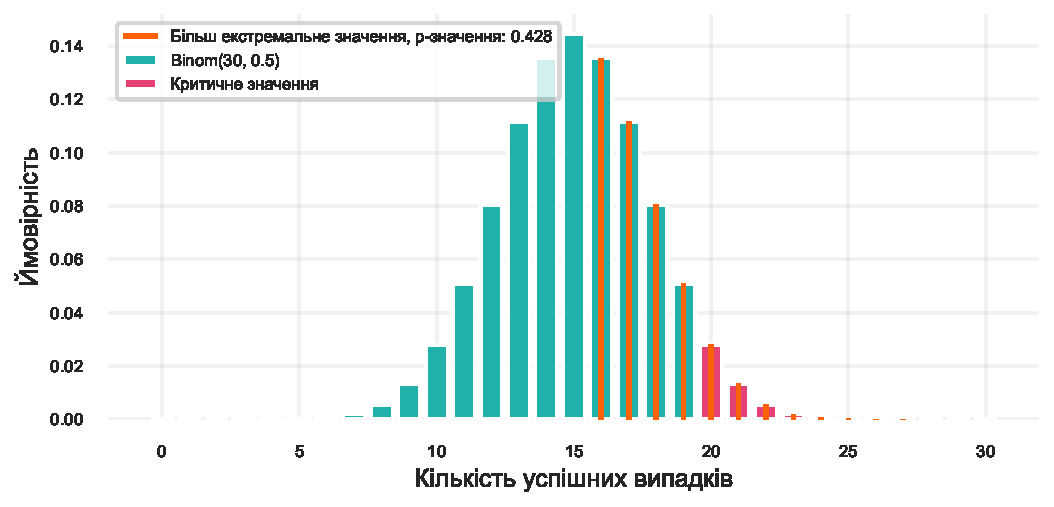
\includegraphics{binom_files/figure-pdf/fig-binom-pmf-p-value-output-1.pdf}

}

\caption{\label{fig-binom-pmf-p-value}\(p\)-значення для критерію
\(Q = 15\)}

\end{figure}%

Тепер виведемо формулу через функції Python:

\[
P_{H_0}(Q \geqslant q) = 1 - P_{H_0}(Q < q) = 1 - F(q)
\]

Зобразимо на графіку область більш екстремальних значень й p-value для
різних значень статистики.

\begin{figure}[H]

\centering{

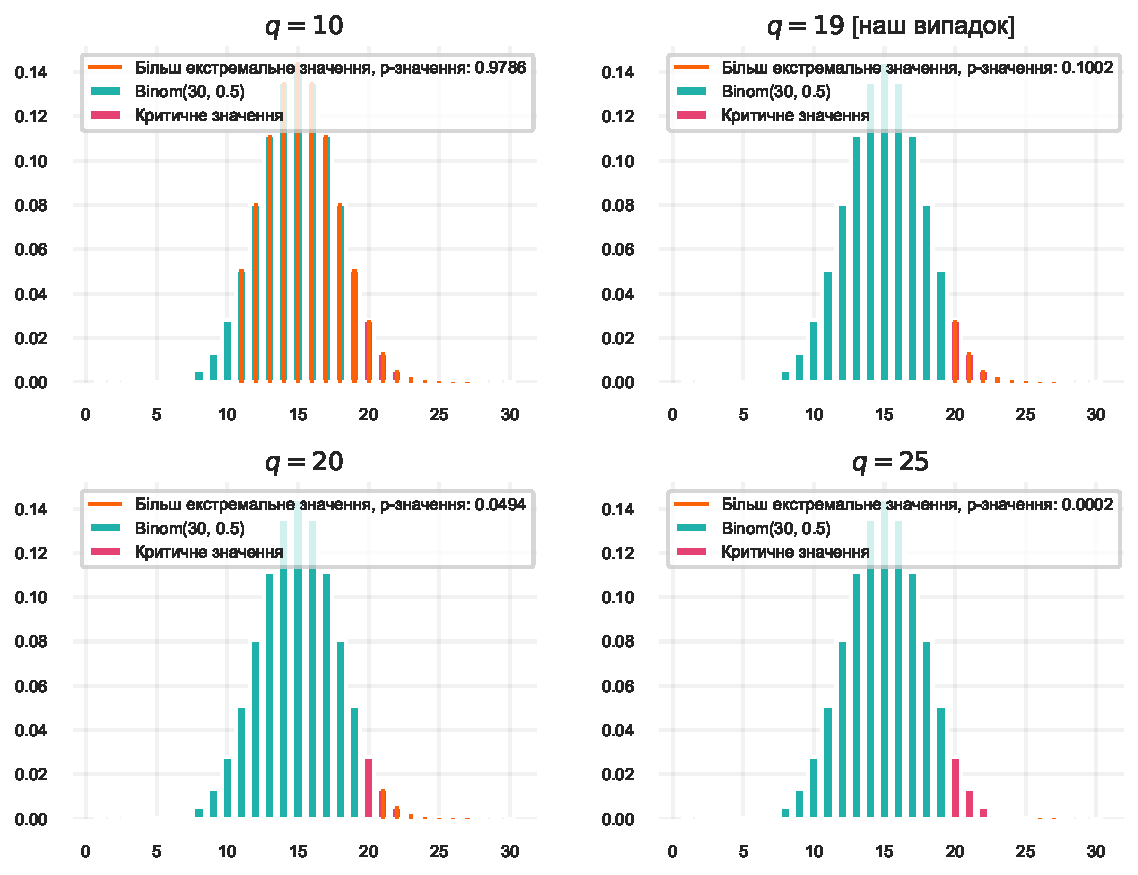
\includegraphics{binom_files/figure-pdf/fig-binom-pmf-p-values-output-1.pdf}

}

\caption{\label{fig-binom-pmf-p-values}\(p\)-значення для критерію
\(Q = 10, 19, 20, 25\)}

\end{figure}%

Можна побачити, що в критичній області \(p\)-значення
\(\leqslant \alpha\), а поза нею \(p\)-значення \(> \alpha\). Саме таке
правило й використовується для прийняття рішення.

\[
H_0 \text{ відкидається } \Leftrightarrow p-значення \leqslant \alpha
\]

Причому за \(p\)-значення одразу видно, що якби в нашу критичну область
включили значення \(19\), наш критерій допускав би FPR у \(10\%\)
випадків, що вже неприпустимо. Тому й гіпотезу ми не відкидаємо.

Зауважимо, що для обчислення \(p\)-значення не знадобилося знання
\(\alpha\), а потрібна була тільки статистика й форма критерію.

\section{Двосторонні
критерії}\label{ux434ux432ux43eux441ux442ux43eux440ux43eux43dux43dux456-ux43aux440ux438ux442ux435ux440ux456ux457}

До цього моменту нас цікавили відхилення від ймовірності в \(50\%\)
тільки в один бік. І логічно, адже це продиктовано бізнесом. Тільки
велика частка успішних підписок призведе до успіху. І зазвичай при
прийнятті рішень так й буває. \textbf{При тестуванні нового рішення або
продукту розглядають альтернативну гіпотезу тільки в бік поліпшення},
тому що в іншому разі немає сенсу впроваджувати рішення на всіх
користувачів.

Однак \textbf{іноді} може знадобитися доводити відхилення в обидва боки,
якщо ви перевіряєте якесь припущення. Нехай вам дали монетку й просять
перевірити, чесна вона чи ні. Монетка чесна, якщо під час підкидання
ймовірність випадання орла дорівнює \(0.5\). Ви підкидаєте монетку
\(30\) разів, кожен кидок --- бернуллівська величина, аналогічно
завданню з сервісом освітніх послуг. Нульова гіпотеза та ж сама:
\(\mu = 0.5\). Але тепер ми хочемо відкидати цю гіпотезу як у разі
великої ймовірності орла, так і в разі маленької, відповідно перевіряємо
\emph{двосторонню гіпотезу}.

\[
H_0: \mu = 0.5
\]

\[
H_1: \mu \neq 0.5
\]

Виберемо критичну область для критерію за такої альтернативи.
Скористаємося тією ж статистикою \(Q(\xi) = \sum \xi_i\). Тільки тепер
відхилення в кожну сторону однаково важливі. Відкидати гіпотезу будемо
не тільки на досить великих значеннях, а й на досить маленьких.
Наприклад, якщо у нас було всього \(2\) орла з \(30\) --- це свідчення
на користь того, що \(\mu \neq 0.5\), але не на користь \(\mu > 0.5\).

Оскільки відхилення в різні боки однаково важливі, а розподіл
симетричний, шукати критерій можна в такому вигляді:

\[
S = \{Q \geqslant C\} \cup \{Q \leqslant n - C\}
\]

\subsection{Як вибрати критичну
область}\label{ux44fux43a-ux432ux438ux431ux440ux430ux442ux438-ux43aux440ux438ux442ux438ux447ux43dux443-ux43eux431ux43bux430ux441ux442ux44c}

Подивимося, який вигляд матиме критична область у такому разі.

\begin{figure}[H]

\centering{

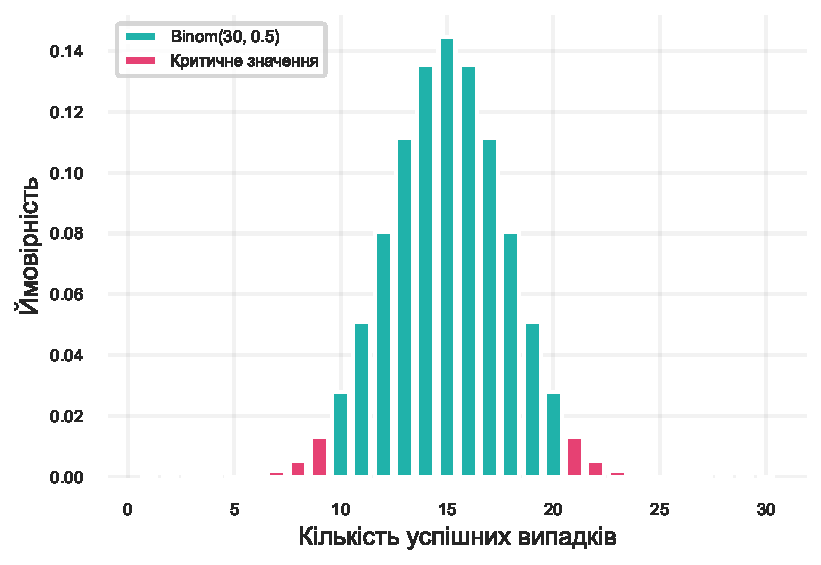
\includegraphics{binom_files/figure-pdf/fig-binom-pmf-two-sided-output-1.pdf}

}

\caption{\label{fig-binom-pmf-two-sided}Двостороння критична область для
критерію \(С = 6\)}

\end{figure}%

З картинки видно, що якщо тепер відкидати відхилення за
\(Q \geqslant 20\), то необхідно відкидати й \(Q \leqslant 10\), а отже,
загальна площа стовпців буде вже приблизно \(0.1\). Тому за рівня
значущості \(0.05\) й \(20\) успіхів гіпотеза вже не відкинеться.

Якщо ж виставити \(C = 6\), то така область уже підходить, площа
стовпців \(\approx 0.043 < 0.05\).

Щоб вибрати порогову константу за формулою, можна помітити, що критична
область симетрична, а значить праворуч площа не повинна бути більшою,
ніж \(\frac{\alpha}{2}\). А таку задачу ми вже вміємо розв'язувати.

Реалізуємо функцію на Python.

\begin{Shaded}
\begin{Highlighting}[]
\KeywordTok{def}\NormalTok{ find\_crit\_subs\_two\_sided(n, mu, alpha):}
    \CommentTok{"""}
\CommentTok{    Знаходить критичне значення для двостороннього критерію}
\CommentTok{    :param n: кількість спостережень}
\CommentTok{    :param mu: ймовірність успіху}
\CommentTok{    :param alpha: рівень значущості}
\CommentTok{    :return: критичне значення}
\CommentTok{    """}
\NormalTok{    binom\_dist }\OperatorTok{=}\NormalTok{ binom(n, mu)}
    \ControlFlowTok{return}\NormalTok{ n }\OperatorTok{/} \DecValTok{2} \OperatorTok{{-}}\NormalTok{ binom\_dist.ppf(alpha }\OperatorTok{/} \DecValTok{2}\NormalTok{) }\OperatorTok{+} \DecValTok{1}
\end{Highlighting}
\end{Shaded}

Використаємо функцію для знаходження критичного значення для
\(\alpha = 0.05\).

\begin{Shaded}
\begin{Highlighting}[]
\NormalTok{find\_crit\_subs\_two\_sided(}\DecValTok{30}\NormalTok{, }\FloatTok{0.5}\NormalTok{, }\FloatTok{0.05}\NormalTok{)}
\end{Highlighting}
\end{Shaded}

\begin{verbatim}
6.0
\end{verbatim}

\subsection{\texorpdfstring{Як знайти
\(p\)-значення}{Як знайти p-значення}}\label{ux44fux43a-ux437ux43dux430ux439ux442ux438-p-ux437ux43dux430ux447ux435ux43dux43dux44f}

Критерій має вигляд

\[
S = \{|Q(\xi) - 15| \geqslant C\}
\]

Позначимо відхилення суми від 15 як \(\Delta(\xi) = |Q(\xi) - 15|\),
тоді ми маємо критерій

\[
S = \{\Delta(\xi) \geqslant C\}
\]

Тобто більш екстремальними вважатимуться ті значення суми, що
знаходяться далі від 15. Щоб обчислити \(p\)-значення, доведеться
порахувати суму площ із двох сторін окремо.

\begin{Shaded}
\begin{Highlighting}[]
\KeywordTok{def}\NormalTok{ pvalue\_two\_sided\_sym(n, q):}
\NormalTok{    binom\_h0 }\OperatorTok{=}\NormalTok{ binom(n}\OperatorTok{=}\NormalTok{n, p}\OperatorTok{=}\FloatTok{0.5}\NormalTok{)}
\NormalTok{    diff }\OperatorTok{=}\NormalTok{ np.}\BuiltInTok{abs}\NormalTok{(q }\OperatorTok{{-}} \DecValTok{15}\NormalTok{)}
\NormalTok{    right\_sq }\OperatorTok{=} \DecValTok{1} \OperatorTok{{-}}\NormalTok{ binom\_h0.cdf(}\DecValTok{15} \OperatorTok{+}\NormalTok{ diff }\OperatorTok{{-}} \DecValTok{1}\NormalTok{)}
\NormalTok{    left\_sq }\OperatorTok{=}\NormalTok{ binom\_h0.cdf(}\DecValTok{15} \OperatorTok{{-}}\NormalTok{ diff)}
    \ControlFlowTok{return}\NormalTok{ left\_sq }\OperatorTok{+}\NormalTok{ right\_sq}
\end{Highlighting}
\end{Shaded}

Насправді через симетричність розподілу ліва і права площа виходять
однаковими, тому можна порахувати площу з одного боку і помножити на 2.

\begin{Shaded}
\begin{Highlighting}[]
\KeywordTok{def}\NormalTok{ pvalue\_two\_sided\_sym\_simple(n, q):}
\NormalTok{    binom\_h0 }\OperatorTok{=}\NormalTok{ binom(n}\OperatorTok{=}\NormalTok{n, p}\OperatorTok{=}\FloatTok{0.5}\NormalTok{)}
\NormalTok{    diff }\OperatorTok{=}\NormalTok{ np.}\BuiltInTok{abs}\NormalTok{(q }\OperatorTok{{-}} \DecValTok{15}\NormalTok{)}
\NormalTok{    right\_sq }\OperatorTok{=} \DecValTok{1} \OperatorTok{{-}}\NormalTok{ binom\_h0.cdf(}\DecValTok{15} \OperatorTok{+}\NormalTok{ diff }\OperatorTok{{-}} \DecValTok{1}\NormalTok{)}
    \ControlFlowTok{return} \DecValTok{2} \OperatorTok{*}\NormalTok{ right\_sq}
\end{Highlighting}
\end{Shaded}

Використаємо функцію для знаходження \(p\)-значення для \(q = 21\).

\begin{Shaded}
\begin{Highlighting}[]
\NormalTok{pvalue\_two\_sided\_sym(}\DecValTok{30}\NormalTok{, }\DecValTok{21}\NormalTok{)}
\end{Highlighting}
\end{Shaded}

\begin{verbatim}
0.04277394525706769
\end{verbatim}

\begin{Shaded}
\begin{Highlighting}[]
\NormalTok{pvalue\_two\_sided\_sym\_simple(}\DecValTok{30}\NormalTok{, }\DecValTok{21}\NormalTok{)}
\end{Highlighting}
\end{Shaded}

\begin{verbatim}
0.04277394525706768
\end{verbatim}

Тепер навіть у разі \(20\) орлів \(p\)-значення \(> 0.05\), тому
відкидати будемо значення, починаючи з \(21\) й менші або такі, що
дорівнюють \(9\).

\subsection{Випадок із несиметричним
розподілом}\label{ux432ux438ux43fux430ux434ux43eux43a-ux456ux437-ux43dux435ux441ux438ux43cux435ux442ux440ux438ux447ux43dux438ux43c-ux440ux43eux437ux43fux43eux434ux456ux43bux43eux43c}

Коли розподіл за справедливості \(H_0\) несиметричний, відхилення від
очікуваного значення в різні боки можуть бути по-різному критичними. Як
приклад розглянемо також біноміальний розподіл, але з імовірністю успіху
\(0.8\).

Тоді можна ліву і праву критичні області побудувати окремо, виділивши на
них по \(\frac{\alpha}{2}\) площі. Праву область ми вже вміємо шукати,
знайдемо ліву.

\begin{Shaded}
\begin{Highlighting}[]
\NormalTok{binom\_h0\_nonsym }\OperatorTok{=}\NormalTok{ binom(n}\OperatorTok{=}\DecValTok{30}\NormalTok{, p}\OperatorTok{=}\FloatTok{0.8}\NormalTok{)}

\NormalTok{probs }\OperatorTok{=}\NormalTok{ binom\_h0\_nonsym.pmf(np.arange(}\DecValTok{31}\NormalTok{))}

\NormalTok{plt.bar(np.arange(}\DecValTok{31}\NormalTok{), probs, color}\OperatorTok{=}\NormalTok{turquoise, label}\OperatorTok{=}\StringTok{"Binom(30, 0.8)"}\NormalTok{)}
\NormalTok{plt.legend(fontsize}\OperatorTok{=}\DecValTok{8}\NormalTok{)}
\NormalTok{plt.show()}
\end{Highlighting}
\end{Shaded}

\begin{figure}[H]

\centering{

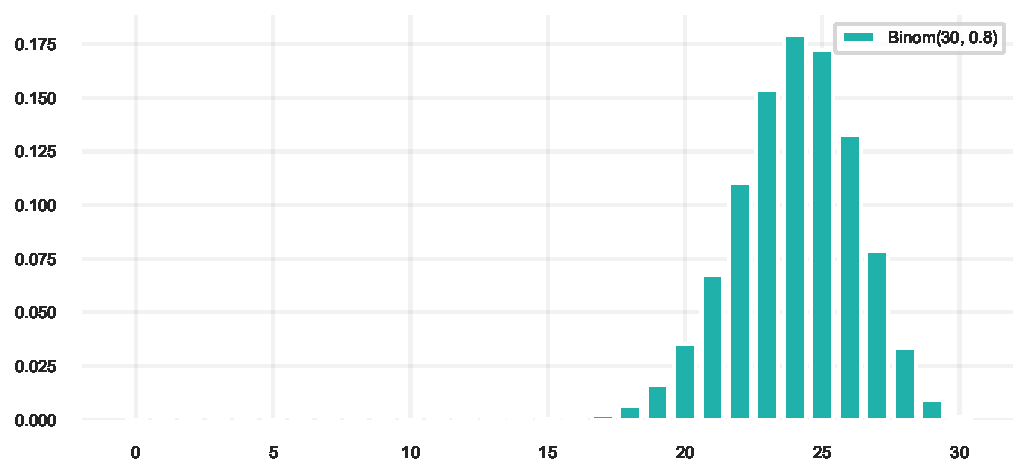
\includegraphics{binom_files/figure-pdf/fig-binom-pmf-two-sided-nonsym-output-1.pdf}

}

\caption{\label{fig-binom-pmf-two-sided-nonsym}Біноміальний розподіл з
імовірністю успіху \(0.8\)}

\end{figure}%

Для того, щоб побудувати двосторонній критерій, потрібно знайти ліворуч
і праворуч області, площа яких становить не більше, ніж
\(\frac{\alpha}{2}\). Для правого боку ми вже розв'язували таку задачу,
розв'яжемо для лівого.

Шукаємо \(C\), таке що

\[
P(Q(\xi) \leqslant C) \leqslant \frac{\alpha}{2}
\]

Спочатку знайдемо перше число, де ймовірність
\(\geqslant \frac{\alpha}{2}\). А це за визначенням
\(\frac{\alpha}{2}\)-квантиль. Достатньо взяти попереднє число, і воно
буде задовольняти нашій умові.

\begin{Shaded}
\begin{Highlighting}[]
\KeywordTok{def}\NormalTok{ two\_sided\_criterion\_nonsym(n, mu, alpha):}
\NormalTok{    binom\_h0 }\OperatorTok{=}\NormalTok{ binom(n}\OperatorTok{=}\NormalTok{n, p}\OperatorTok{=}\NormalTok{mu)}
\NormalTok{    c2 }\OperatorTok{=}\NormalTok{ binom\_h0.ppf(}\DecValTok{1} \OperatorTok{{-}}\NormalTok{ alpha}\OperatorTok{/}\DecValTok{2}\NormalTok{) }\OperatorTok{+} \DecValTok{1}
\NormalTok{    c1 }\OperatorTok{=}\NormalTok{ binom\_h0.ppf(alpha}\OperatorTok{/}\DecValTok{2}\NormalTok{) }\OperatorTok{{-}} \DecValTok{1}
    \ControlFlowTok{return}\NormalTok{ c1, c2}
\end{Highlighting}
\end{Shaded}

Використаємо функцію для знаходження критичних значень для
\(\alpha = 0.05\).

\begin{Shaded}
\begin{Highlighting}[]
\NormalTok{two\_sided\_criterion\_nonsym(}\DecValTok{30}\NormalTok{, }\FloatTok{0.8}\NormalTok{, }\FloatTok{0.05}\NormalTok{)}
\end{Highlighting}
\end{Shaded}

\begin{verbatim}
(18.0, 29.0)
\end{verbatim}

Отже, наш критерій для перевірки гіпотези

\[
H_0: \mu = 0.8
\]

\[
H_1: \mu \neq 0.8
\]

має вигляд

\[
S = \{Q(\xi) \leqslant 18\} \cup \{Q(\xi) \geqslant 29\}
\]

Тут межа \(29\) уже має логічний вигляд, бо треба спростувати 80\%
орлів/успіхів, а для цього потрібна велика їхня кількість.

Зобразимо критичну область на графіку.

\begin{Shaded}
\begin{Highlighting}[]
\NormalTok{C1, C2 }\OperatorTok{=}\NormalTok{ two\_sided\_criterion\_nonsym(}\DecValTok{30}\NormalTok{, }\FloatTok{0.8}\NormalTok{, }\FloatTok{0.05}\NormalTok{)}

\NormalTok{plt.figure(figsize}\OperatorTok{=}\NormalTok{(}\DecValTok{6}\NormalTok{, }\DecValTok{4}\NormalTok{))}
\NormalTok{plt.bar(np.arange(}\DecValTok{31}\NormalTok{), probs, color}\OperatorTok{=}\NormalTok{turquoise, label}\OperatorTok{=}\StringTok{"Binom(30, 0.8)"}\NormalTok{)}
\NormalTok{plt.bar(np.arange(}\DecValTok{31}\NormalTok{)[np.arange(}\DecValTok{31}\NormalTok{) }\OperatorTok{\textless{}=}\NormalTok{ C1], probs[np.arange(}\DecValTok{31}\NormalTok{) }\OperatorTok{\textless{}=}\NormalTok{ C1], color}\OperatorTok{=}\NormalTok{red\_pink, label}\OperatorTok{=}\StringTok{"Критичне значення"}\NormalTok{)}
\NormalTok{plt.bar(np.arange(}\DecValTok{31}\NormalTok{)[np.arange(}\DecValTok{31}\NormalTok{) }\OperatorTok{\textgreater{}=}\NormalTok{ C2], probs[np.arange(}\DecValTok{31}\NormalTok{) }\OperatorTok{\textgreater{}=}\NormalTok{ C2], color}\OperatorTok{=}\NormalTok{red\_pink)}
\NormalTok{plt.xlabel(}\StringTok{"Кількість успішних випадків"}\NormalTok{)}
\NormalTok{plt.ylabel(}\StringTok{"Ймовірність"}\NormalTok{)}
\NormalTok{plt.legend(fontsize }\OperatorTok{=} \StringTok{\textquotesingle{}8\textquotesingle{}}\NormalTok{, loc }\OperatorTok{=} \StringTok{\textquotesingle{}upper left\textquotesingle{}}\NormalTok{)}
\NormalTok{plt.show()}
\end{Highlighting}
\end{Shaded}

\begin{figure}[H]

\centering{

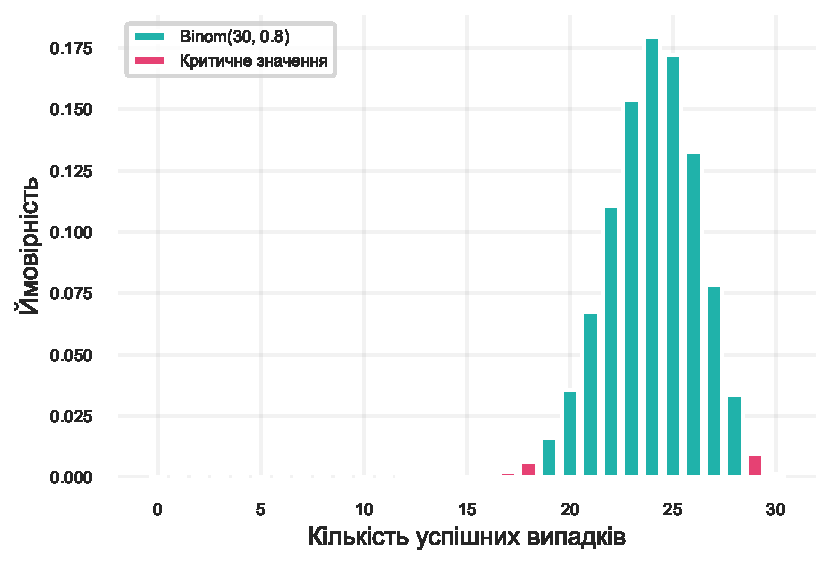
\includegraphics{binom_files/figure-pdf/fig-binom-pmf-two-sided-nonsym-crit-output-1.pdf}

}

\caption{\label{fig-binom-pmf-two-sided-nonsym-crit}Двостороння критична
область для критерію \(C_1 = 18, C_2 = 29\)}

\end{figure}%

\subsection{\texorpdfstring{\(p\)-значення для несиметричного
розподілу}{p-значення для несиметричного розподілу}}\label{p-ux437ux43dux430ux447ux435ux43dux43dux44f-ux434ux43bux44f-ux43dux435ux441ux438ux43cux435ux442ux440ux438ux447ux43dux43eux433ux43e-ux440ux43eux437ux43fux43eux434ux456ux43bux443}

Цей критерій --- об'єднання двох критеріїв рівня значущості
\(\frac{\alpha}{2}\), для кожного з яких можна порахувати
\(p\)-значення. Позначимо їх як \(p_1, p_2\). Перший критерій
відкидається при \(p_1 \leqslant \frac{\alpha}{2}\), другий при
\(p_2 \leqslant \frac{\alpha}{2}\). А наш об'єднаний, коли виконано одну
з цих умов, тобто

\[
2p_1 \leqslant \alpha \vee 2p_2 \leqslant \alpha \Leftrightarrow 2 \cdot \min(p_1, p_2) \leqslant \alpha
\]

Отже, можна рахувати \(p\)-значення як \(2 \min(p_1, p_2)\) й
порівнювати з \(\alpha\).

Проведемо аналогію із симетричним випадком: якщо сума опинилася в лівій
частині, то потрібно порахувати \(p\)-значення лівого критерію і
помножити на 2. Якщо сума опинилася в правій частині, то потрібно
порахувати \(p\)-значення правого критерію і помножити на 2.

\begin{Shaded}
\begin{Highlighting}[]
\KeywordTok{def}\NormalTok{ pvalue\_two\_sided(n, q, mu}\OperatorTok{=}\FloatTok{0.5}\NormalTok{):}
\NormalTok{    binom\_h0 }\OperatorTok{=}\NormalTok{ binom(n}\OperatorTok{=}\NormalTok{n, p}\OperatorTok{=}\NormalTok{mu)}
\NormalTok{    pvalue\_left }\OperatorTok{=}\NormalTok{ binom\_h0.cdf(q)}
\NormalTok{    pvalue\_right }\OperatorTok{=} \DecValTok{1} \OperatorTok{{-}}\NormalTok{ binom\_h0.cdf(q }\OperatorTok{{-}} \DecValTok{1}\NormalTok{)}
    \ControlFlowTok{return} \DecValTok{2} \OperatorTok{*} \BuiltInTok{min}\NormalTok{(pvalue\_left, pvalue\_right)}
\end{Highlighting}
\end{Shaded}

Використаємо функцію для знаходження \(p\)-значення для \(q = 28\).

\begin{Shaded}
\begin{Highlighting}[]
\NormalTok{pvalue\_two\_sided(}\DecValTok{30}\NormalTok{, }\DecValTok{28}\NormalTok{, }\FloatTok{0.8}\NormalTok{)}
\end{Highlighting}
\end{Shaded}

\begin{verbatim}
0.08835797030399428
\end{verbatim}

Видно, що \(p\)-значення \(> 0.05\), отже, на рівні значущості \(0.05\)
навіть \(28\) успіхів недостатньо, щоб відкинути ймовірність успіху в
\(80\%\).

Зауважимо, що ця ж функція працює і для симетричного випадку, повертаючи
той самий результат.

\begin{Shaded}
\begin{Highlighting}[]
\NormalTok{pvalue\_two\_sided(n}\OperatorTok{=}\DecValTok{30}\NormalTok{, q}\OperatorTok{=}\DecValTok{20}\NormalTok{, mu}\OperatorTok{=}\FloatTok{0.5}\NormalTok{)}
\end{Highlighting}
\end{Shaded}

\begin{verbatim}
0.09873714670538902
\end{verbatim}

\begin{Shaded}
\begin{Highlighting}[]
\NormalTok{pvalue\_two\_sided\_sym(n}\OperatorTok{=}\DecValTok{30}\NormalTok{, q}\OperatorTok{=}\DecValTok{20}\NormalTok{)}
\end{Highlighting}
\end{Shaded}

\begin{verbatim}
0.09873714670538904
\end{verbatim}

\section{Готові
функції}\label{ux433ux43eux442ux43eux432ux456-ux444ux443ux43dux43aux446ux456ux457}

Звісно, можна використати готові функції з бібліотеки \texttt{scipy}.
Для цього використаємо функцію \texttt{binomtest}, котра має параметри:

\begin{itemize}
\tightlist
\item
  \texttt{k} --- кількість успіхів
\item
  \texttt{n} --- кількість спостережень
\item
  \texttt{p} --- ймовірність успіху
\item
  \texttt{alternative} --- тип гіпотези:

  \begin{itemize}
  \tightlist
  \item
    \texttt{two-sided}: двостороння
  \item
    \texttt{greater}: правостороння
  \item
    \texttt{less}: лівостороння
  \end{itemize}
\end{itemize}

\begin{Shaded}
\begin{Highlighting}[]
\ImportTok{from}\NormalTok{ scipy.stats }\ImportTok{import}\NormalTok{ binomtest}

\NormalTok{result }\OperatorTok{=}\NormalTok{ binomtest(}\DecValTok{19}\NormalTok{, }\DecValTok{30}\NormalTok{, }\FloatTok{0.5}\NormalTok{, alternative}\OperatorTok{=}\StringTok{\textquotesingle{}two{-}sided\textquotesingle{}}\NormalTok{)}

\BuiltInTok{print}\NormalTok{(}\SpecialStringTok{f"Статистика: }\SpecialCharTok{\{}\NormalTok{result}\SpecialCharTok{.}\NormalTok{statistic}\SpecialCharTok{\}}\SpecialStringTok{"}\NormalTok{)}
\BuiltInTok{print}\NormalTok{(}\SpecialStringTok{f"p{-}значення: }\SpecialCharTok{\{}\NormalTok{result}\SpecialCharTok{.}\NormalTok{pvalue}\SpecialCharTok{\}}\SpecialStringTok{"}\NormalTok{)}
\end{Highlighting}
\end{Shaded}

\begin{verbatim}
Статистика: 0.6333333333333333
p-значення: 0.20048842206597334
\end{verbatim}

\section{Статистична
потужність}\label{ux441ux442ux430ux442ux438ux441ux442ux438ux447ux43dux430-ux43fux43eux442ux443ux436ux43dux456ux441ux442ux44c}

\subsection{Хибно негативні
помилки}\label{ux445ux438ux431ux43dux43e-ux43dux435ux433ux430ux442ux438ux432ux43dux456-ux43fux43eux43cux438ux43bux43aux438}

Раніше під час побудови критеріїв ми звертали увагу тільки на
\(\alpha\), рівень значущості критерію. Але цей параметр контролює лише
хибнопозитивну помилку (False Positive), а саме ймовірність, що критерій
прийме \(H_1\) за умови вірності \(H_0\).

Але є ще один вид помилок, які може допустити критерій --- хибно
негативні помилки (False Negative). Це випадки, коли критерій приймає
\(H_0\) за умови вірності \(H_1\). Це важливо, оскільки вони можуть
вказувати на те, що критерій не чутливий до змін, які відбуваються в
даних.

Випадок, коли ймовірність FPR \(< \alpha\), але при цьому ймовірність
хибно негативні помилки (False Negative Rate, FNR) величезна, можна
навести легко. Для цього достатньо \textbf{ніколи} не відкидати
гіпотезу, взявши критерій \(S \equiv 0\).

Наведемо приклад, коли помилки False Negative відбуваються не завжди,
але критерії є все одно нечутливими.

\subsection{Критерій пори
року}\label{ux43aux440ux438ux442ux435ux440ux456ux439-ux43fux43eux440ux438-ux440ux43eux43aux443}

Поставимо гіпотезу про те, що зараз на вулиці літо. Для перевірки можна
було б, звісно, подивитися в календар, але ми зробимо інакше.

\[
H_0: \text{ на вулиці літо}
\]

\[
H_1: \text{ на вулиці не літо}
\]

Подивимося у вікно і визначимо, чи йде там сніг. Якщо він йде, то це
непоганий доказ того, що зараз не літо, а отже можна відкинути \(H_0\).

Порахуємо FPR та FNR для цього критерію. Ми знаємо, що влітку сніг іде
дуже рідко (ймовірність помилки нижча за \(0.1\%\)), тож це точно
критерій рівня значущості \(0.001\), чого зазвичай достатньо для
критеріїв.

\[
FPR(S) = P(\text{йде сніг}\ |\ \text{сьогодні літо}) < 0.001
\]

Але що з FNR? Розглянемо конкретний випадок: зараз вересень. Оскільки у
вересні майже завжди немає снігу, можна сказати, що FNR більша за
\(90\%\), отже, цей критерій насправді мало дієвий.

\[
FNR(S) = P(\text{не йде сніг}\ |\ \text{зараз вересень}) > 0.9
\]

Сформулюємо інший критерій рівня значущості \(\alpha\), причому в цьому
разі рівень значущості можна вибрати довільним.

\[
S(\xi) = \begin{cases}
    1, \text{ якщо монетка з імовірністю орла } \alpha \text{ випала орлом} \\
    0, \text{ інакше}
\end{cases}
\]

Виходить, цей критерій випадковий, і він не використовує взагалі жодної
інформації про погоду. Однак вимогам до рівня значущості він
задовольняє.

\[
FPR = P(\text{випав орел}\ |\ \text{сьогодні літо}) = P(\text{випав орел}) = \alpha
\]

Обчислимо FNR.

\[
FNR = P(\text{не випав орел}\ |\ \text{сьогодні не літо}) = P(\text{не випав орел}) = 1 - \alpha
\]

За \(\alpha = 0.001\), як у першому випадку, отримуємо ймовірність FNR
\(0.999 > 0.9\), тобто за однакового рівня значущості з першим
критерієм, другий критерій частіше припускається хибно негативної
помилки.

\subsection{Потужність}\label{ux43fux43eux442ux443ux436ux43dux456ux441ux442ux44c}

У статистиці заведено позитивним результатом вважати відкидання нульової
гіпотези, бо зазвичай підтвердження альтернативи означає наявність
бізнес-результату. Тому вважається хорошим критерій, який частіше дає
змогу виявити бізнес-результат. І рахують тоді не ймовірність хибно
негативної помилки, а \emph{потужність}, що дорівнює ймовірності
відкинути нульову гіпотезу за вірності \(H_1\), тобто ймовірність
\textbf{істинно позитивного результату} (True Positive Rate, TPR).

\begin{equation}\phantomsection\label{eq-power}{
\text{Power}_S = 1 - FNR
}\end{equation}

Коли альтернатива \(H_1\) складається з множини результатів, потужність
розглядають як функцію від результату. Наприклад, можна порахувати
потужність першого та другого критеріїв взимку й восени.

\[
\text{Power}_S(\mu) = 1 - FNR(\mu)
\]

\textbf{Перший критерій}

\[
\text{Power}_S(\text{травень}) = P(\text{їде сніг } | \text{ травень}) \approx 0.00001
\]

\[
\text{Power}_S(\text{жовтень}) = P(\text{їде сніг } | \text{ жовтень}) \approx 0.1
\]

\[
\text{Power}_S(\text{січень}) = P(\text{їде сніг } | \text{ січень}) \approx 0.5
\]

\textbf{Другий критерій}

\[
\text{Power}_S(\text{травень}) = P(\text{випав орел } | \text{ травень}) = \alpha = 0.001
\]

\[
\text{Power}_S(\text{жовтень}) = P(\text{випав орел } | \text{ жовтень}) = \alpha = 0.001
\]

\[
\text{Power}_S(\text{січень}) = P(\text{випав орел } | \text{ січень}) = \alpha = 0.001
\]

Зазвичай завдання пошуку найкращого критерію формулюється як пошук
якомога потужнішого критерію за заданого рівня значущості
\(FPR \leqslant \alpha\). Але ми сказали, що потужність --- функція від
параметра, у нашому випадку від місяця.

Якщо ми застосовуватимемо критерій у січні, то потужнішим буде перший
критерій, а якщо в травні, то потужнішим буде другий критерій. Тому
потрібно розуміти, коли буде застосовуватися критерій, а отже, ми
шукаємо найпотужніший критерій у галузі, яка нас цікавить.

Хоча в реальності в травні потужність обох критеріїв настільки низька,
що вони просто не приносять користі, й використовувати їх не має сенсу.

\section{Потужність для біноміального
розподілу}\label{ux43fux43eux442ux443ux436ux43dux456ux441ux442ux44c-ux434ux43bux44f-ux431ux456ux43dux43eux43cux456ux430ux43bux44cux43dux43eux433ux43e-ux440ux43eux437ux43fux43eux434ux456ux43bux443}

Застосуємо нові знання про потужність для нашої задачі з освітнім
сервісом. З бізнес-міркувань ми вже вибрали \(\alpha = 0.05\), а отже,
знаємо, що ми неправильно відкидаємо гіпотезу \(H_0:\ \mu = 0.5\) з
ймовірністю не більше, ніж \(5\%\). Тобто цим обмежена ймовірність хибно
позитивної помилки.

А з якою ймовірністю ми будемо \emph{правильно} відкидати гіпотезу? І
яка в нас буде ймовірність хибно негативної помилки? На це запитання
якраз відповість формула потужності.

Згадаймо критерій, за яким ми приймаємо рішення:

\[
Q(\xi) = \sum\limits_{i=1}^n \xi_i - \text{кількість підписок}
\]

\[
S = \{Q \geqslant 20\}
\]

Тобто якщо отримуємо хоча б \(20\) успішних підписок, то відкидаємо
\({H}_0\).

Зауважимо, що потужність залежить від того, яке значення \(\mu\) у нашій
генеральній сукупності. Зафіксуємо спочатку параметр \(\mu = 0.6\) й
порахуємо потужність для нього. Якщо істинний параметр такий, то
статистика \(Q\) має розподіл \(Binom(30, 0.6)\).

\begin{Shaded}
\begin{Highlighting}[]
\NormalTok{binom\_h0 }\OperatorTok{=}\NormalTok{ binom(n}\OperatorTok{=}\DecValTok{30}\NormalTok{, p}\OperatorTok{=}\FloatTok{0.5}\NormalTok{)}
\NormalTok{binom\_alternative }\OperatorTok{=}\NormalTok{ binom(n}\OperatorTok{=}\DecValTok{30}\NormalTok{, p}\OperatorTok{=}\FloatTok{0.6}\NormalTok{)}

\NormalTok{x\_grid }\OperatorTok{=}\NormalTok{ np.arange(}\DecValTok{1}\NormalTok{, }\DecValTok{31}\NormalTok{)}
\NormalTok{crit\_reg }\OperatorTok{=}\NormalTok{ x\_grid }\OperatorTok{\textgreater{}=} \DecValTok{20}

\NormalTok{probs\_h0 }\OperatorTok{=}\NormalTok{ binom\_h0.pmf(x\_grid)}
\NormalTok{plt.bar(x\_grid, probs\_h0, color}\OperatorTok{=}\NormalTok{turquoise, label}\OperatorTok{=}\StringTok{\textquotesingle{}PMF, $Binom(0.5, 30)$\textquotesingle{}}\NormalTok{)}

\NormalTok{probs\_alternative }\OperatorTok{=}\NormalTok{ binom\_alternative.pmf(x\_grid)}
\NormalTok{plt.bar(x\_grid, probs\_alternative, color}\OperatorTok{=}\NormalTok{slate, label}\OperatorTok{=}\StringTok{\textquotesingle{}PMF, $Binom(0.6, 30)$\textquotesingle{}}\NormalTok{)}
\NormalTok{plt.bar(x\_grid[crit\_reg], probs\_alternative[crit\_reg], color}\OperatorTok{=}\NormalTok{red\_pink, label}\OperatorTok{=}\StringTok{\textquotesingle{}Критична область\textquotesingle{}}\NormalTok{)}

\NormalTok{plt.legend(fontsize}\OperatorTok{=}\DecValTok{8}\NormalTok{)}
\NormalTok{plt.show()}
\end{Highlighting}
\end{Shaded}

\begin{figure}[H]

\centering{

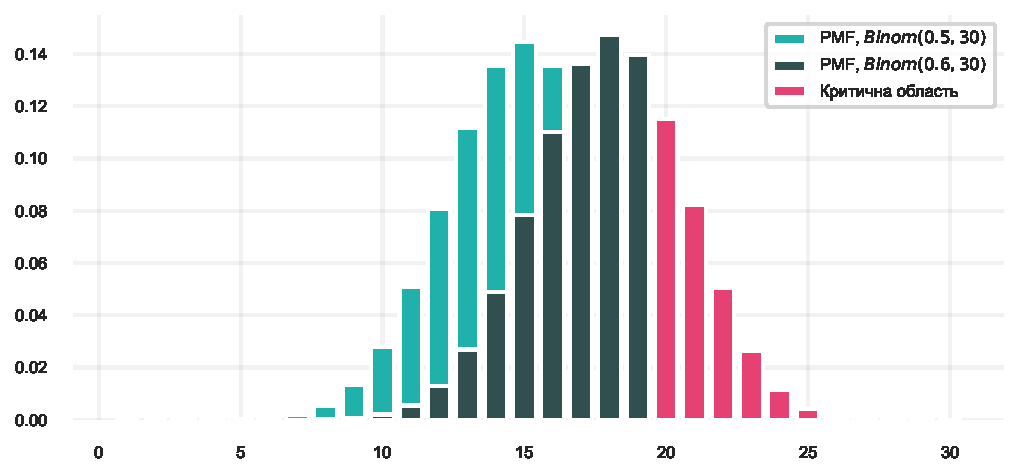
\includegraphics{binom_files/figure-pdf/fig-binom-power-output-1.pdf}

}

\caption{\label{fig-binom-power}Потужність критерію для \(\mu = 0.6\)}

\end{figure}%

Як і раніше, нас цікавить імовірність отримати \(20\) або більше
успіхів. Але якщо раніше ми дивилися на неї для розподілу з \(\mu=0.5\)
й хотіли, щоб вона була меншою за \(5\%\), то тепер ми дивимося за
\(\mu = 0.6\) та прагнемо зробити цю величину якомога більшою. Порівняно
з обчисленням FPR формула не зміниться, змінюється тільки \(\mu\)

\begin{codelisting}

\caption{\label{lst-binom-power}Обчислення потужності критерію}

\centering{

\begin{Shaded}
\begin{Highlighting}[]
\NormalTok{critical\_value }\OperatorTok{=} \DecValTok{20}
\NormalTok{power }\OperatorTok{=} \DecValTok{1} \OperatorTok{{-}}\NormalTok{ binom(n}\OperatorTok{=}\DecValTok{30}\NormalTok{, p}\OperatorTok{=}\FloatTok{0.6}\NormalTok{).cdf(critical\_value }\OperatorTok{{-}} \DecValTok{1}\NormalTok{)}
\NormalTok{fpr   }\OperatorTok{=} \DecValTok{1} \OperatorTok{{-}}\NormalTok{ binom(n}\OperatorTok{=}\DecValTok{30}\NormalTok{, p}\OperatorTok{=}\FloatTok{0.5}\NormalTok{).cdf(critical\_value }\OperatorTok{{-}} \DecValTok{1}\NormalTok{)}

\BuiltInTok{print}\NormalTok{(}\SpecialStringTok{f"Хибно позитивна помилка: }\SpecialCharTok{\{}\NormalTok{fpr}\SpecialCharTok{:.1\%\}}\SpecialStringTok{"}\NormalTok{)}
\BuiltInTok{print}\NormalTok{(}\SpecialStringTok{f"Потужність: }\SpecialCharTok{\{}\NormalTok{power}\SpecialCharTok{:.1\%\}}\SpecialStringTok{"}\NormalTok{)}
\end{Highlighting}
\end{Shaded}

}

\end{codelisting}%

\begin{verbatim}
Хибно позитивна помилка: 4.9%
Потужність: 29.1%
\end{verbatim}

\section{Висновок}\label{ux432ux438ux441ux43dux43eux432ux43eux43a}

Ми розглянули, як можна використовувати біноміальний розподіл для
перевірки гіпотези про ймовірність успіху. Для цього ми визначили
критерій, критичну область, \(p\)-значення. Показали, як можна
використовувати ці поняття для різних видів гіпотез: односторонніх,
двосторонніх, симетричних та несиметричних.

\section{Питання для
самоперевірки}\label{ux43fux438ux442ux430ux43dux43dux44f-ux434ux43bux44f-ux441ux430ux43cux43eux43fux435ux440ux435ux432ux456ux440ux43aux438}

\begin{enumerate}
\def\labelenumi{\arabic{enumi}.}
\tightlist
\item
  Які гіпотези можна перевірити за допомогою біноміального розподілу?
\item
  Як визначити критичну область для критерію?
\item
  Як визначити \(p\)-значення для критерію?
\item
  Як визначити критичну область для двостороннього критерію?
\item
  Як визначити \(p\)-значення для двостороннього критерію?
\item
  Як визначити критичну область для несиметричного розподілу?
\item
  Як визначити \(p\)-значення для несиметричного розподілу?
\end{enumerate}

\bookmarksetup{startatroot}

\chapter{\texorpdfstring{\(Z\)-критерій
Фішера}{Z-критерій Фішера}}\label{sec-z-test}

\bookmarksetup{startatroot}

\chapter{\texorpdfstring{\(t\)-критерій
Стьюдента}{t-критерій Стьюдента}}\label{sec-t-test}

\bookmarksetup{startatroot}

\chapter{Монте-Карло в задачах статистики}\label{sec-monte-carlo}

\bookmarksetup{startatroot}

\chapter*{Підсумки}\label{ux43fux456ux434ux441ux443ux43cux43aux438}
\addcontentsline{toc}{chapter}{Підсумки}

\markboth{Підсумки}{Підсумки}




\end{document}
